\section{Netztopologien}

\subsection{Strahlnetz}
    \begin{minipage}[t]{0.5\columnwidth}
        \begin{itemize}
            \pro geringer Planungsaufwand
            \pro große Übersichtlichkeit bei der Fehlersuche
            \pro geringe Anforderungen an den Netzschutz
            \vspace{1em}
            \con größer werdende Spannungsabfälle mit zunehmendem Abstand von der Einspeisung
            \con höhere Leistungsverluste mit zunehmendem Abstand von der Einspeisung
        \end{itemize}
    \end{minipage}%
    \hfill
    \begin{minipage}[t]{0.45\columnwidth}
        \centering \vspace{-0.7\baselineskip}
        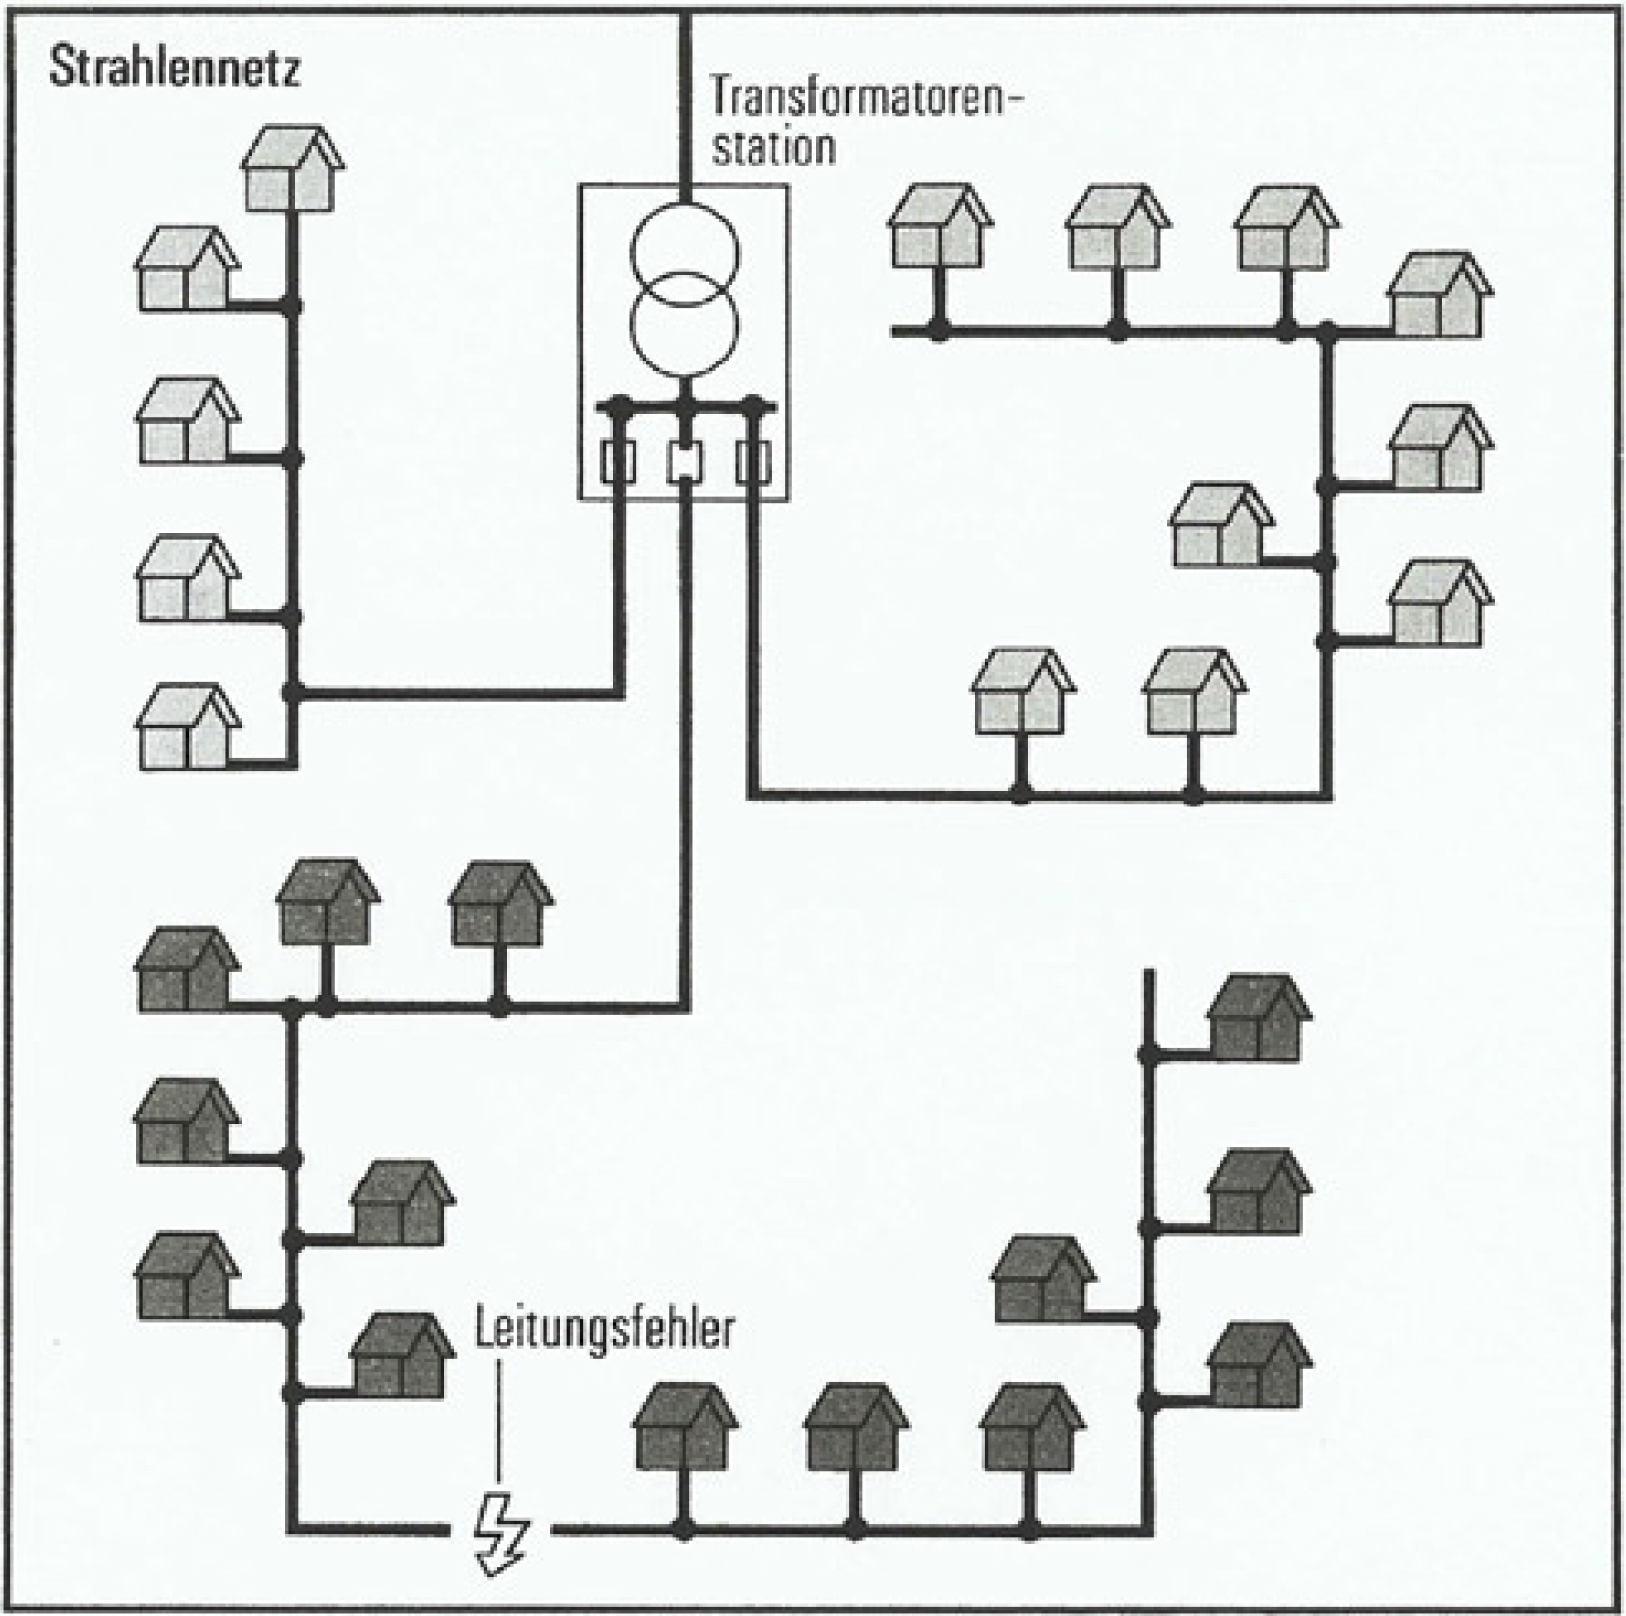
\includegraphics[width=0.9\textwidth]{images/Strahlnetz.png}
    \end{minipage}

% \textbf{Pro:}
%     \begin{itemize}
%         \item geringer Planungsaufwand
%         \item große Übersichtlichkeit bei der Fehlersuche
%         \item geringe Anforderungen an den Netzschutz
%     \end{itemize}
% \vspace{1em}
% \textbf{Contra:}
%     \begin{itemize}
%         \item größer werdende Spannungsabfälle mit zunehmendem Abstand von der Einspeisung
%         \item höhere Leistungsverluste mit zunehmendem Abstand von der Einspeisung
%     \end{itemize}

\subsection{Ringnetz}
    \begin{minipage}[t]{0.5\columnwidth}
        \begin{itemize}
            \pro höhere Versorgungssicherheit
            \pro geringere Verluste
            \pro verbesserte Spannungshaltung
            \vspace{1em}
            \con höhere Anspruch an die Qualifikation des Wartungspersonals
        \end{itemize}
    \end{minipage}%
    \hfill
    \begin{minipage}[t]{0.45\columnwidth}
        \centering \vspace{-0.7\baselineskip}
        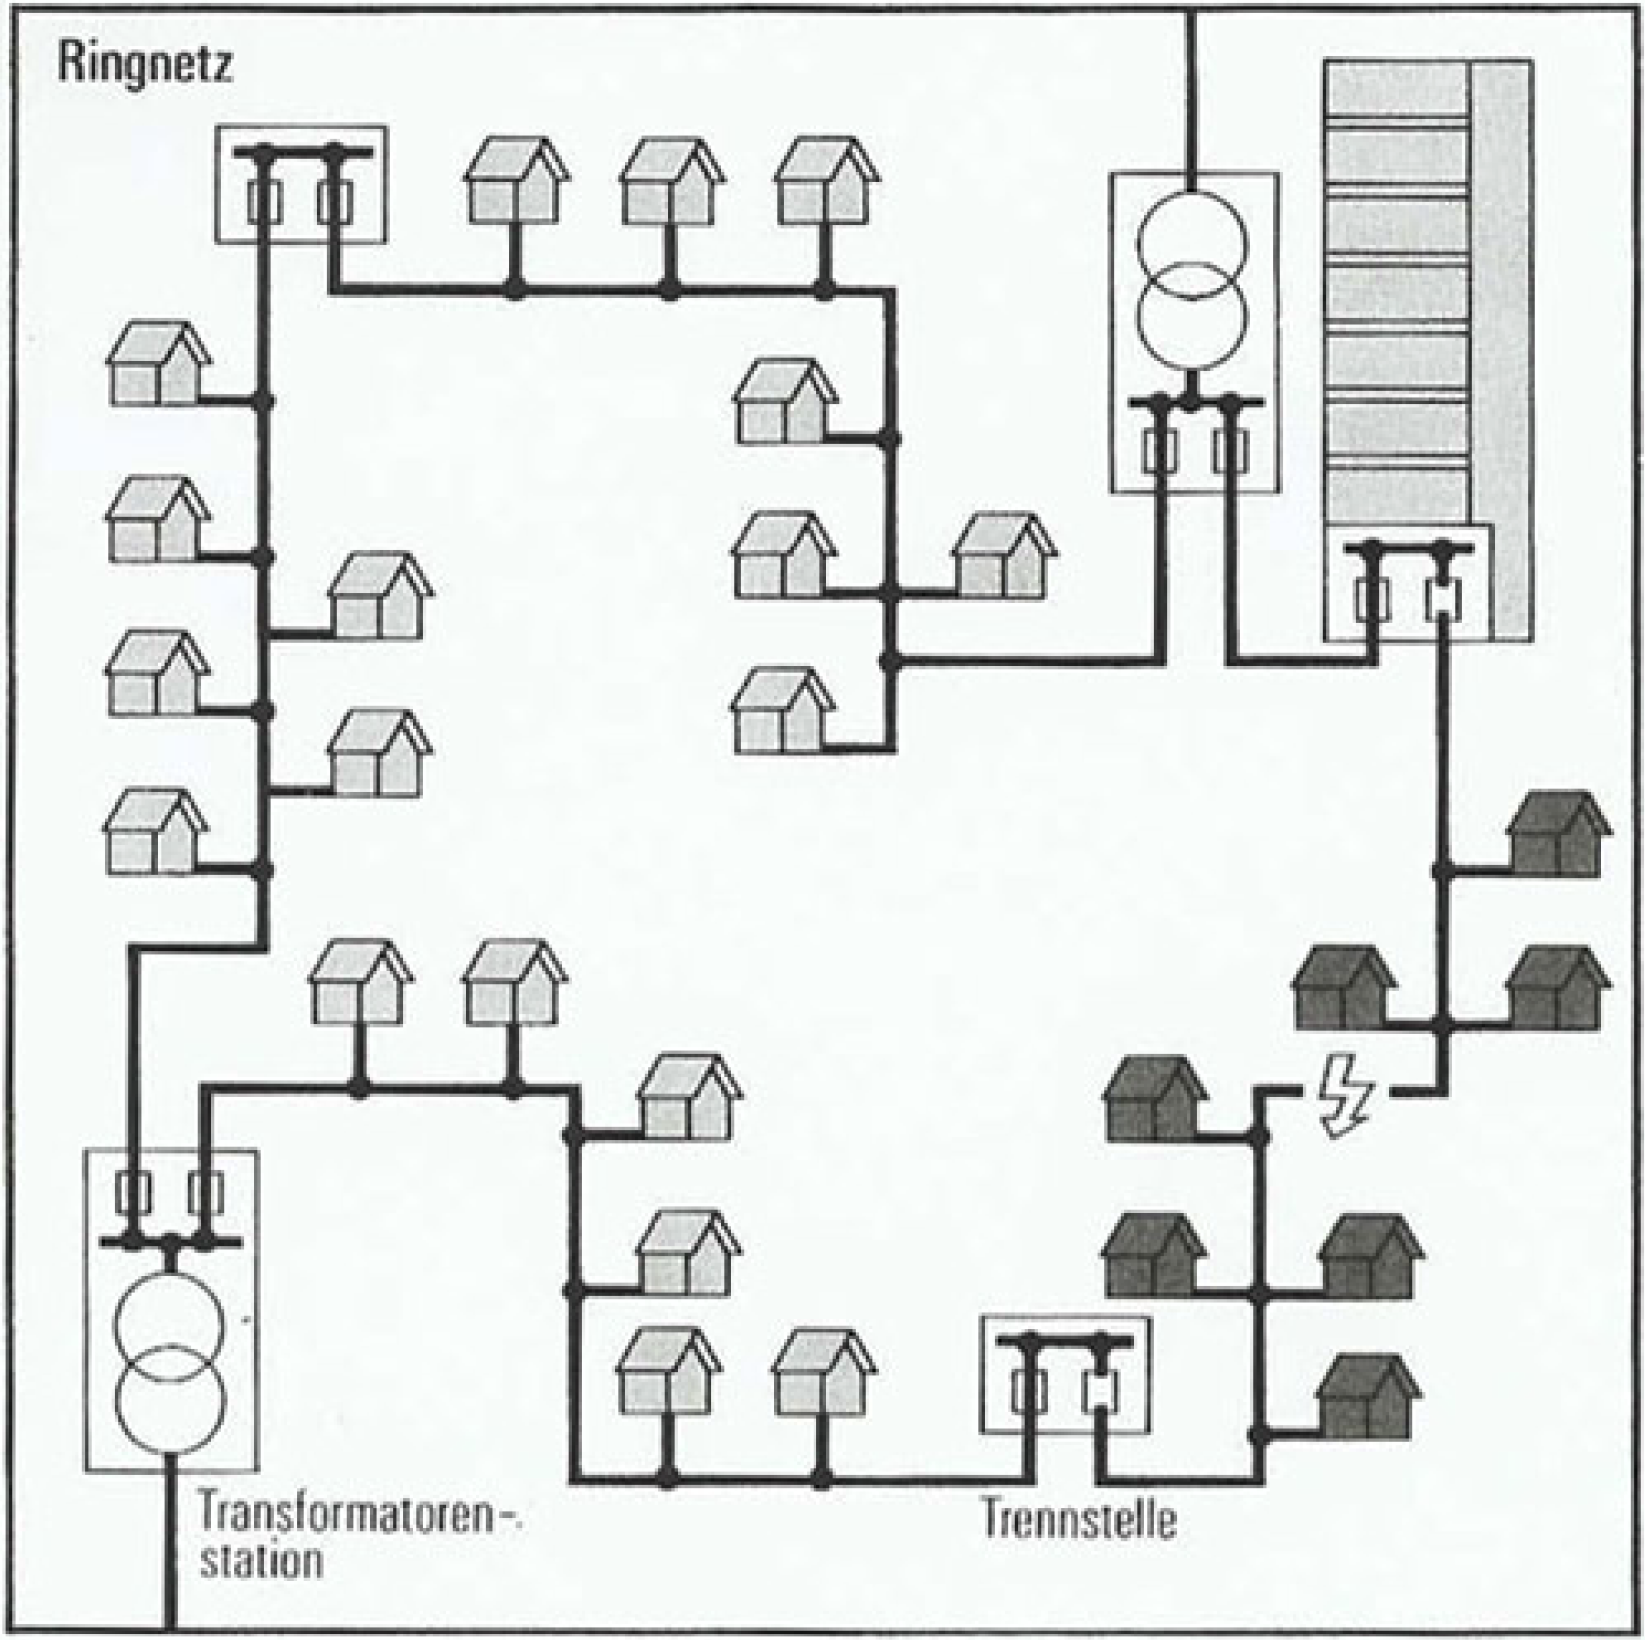
\includegraphics[width=0.9\textwidth]{images/Ringnetz.png}
    \end{minipage}

% 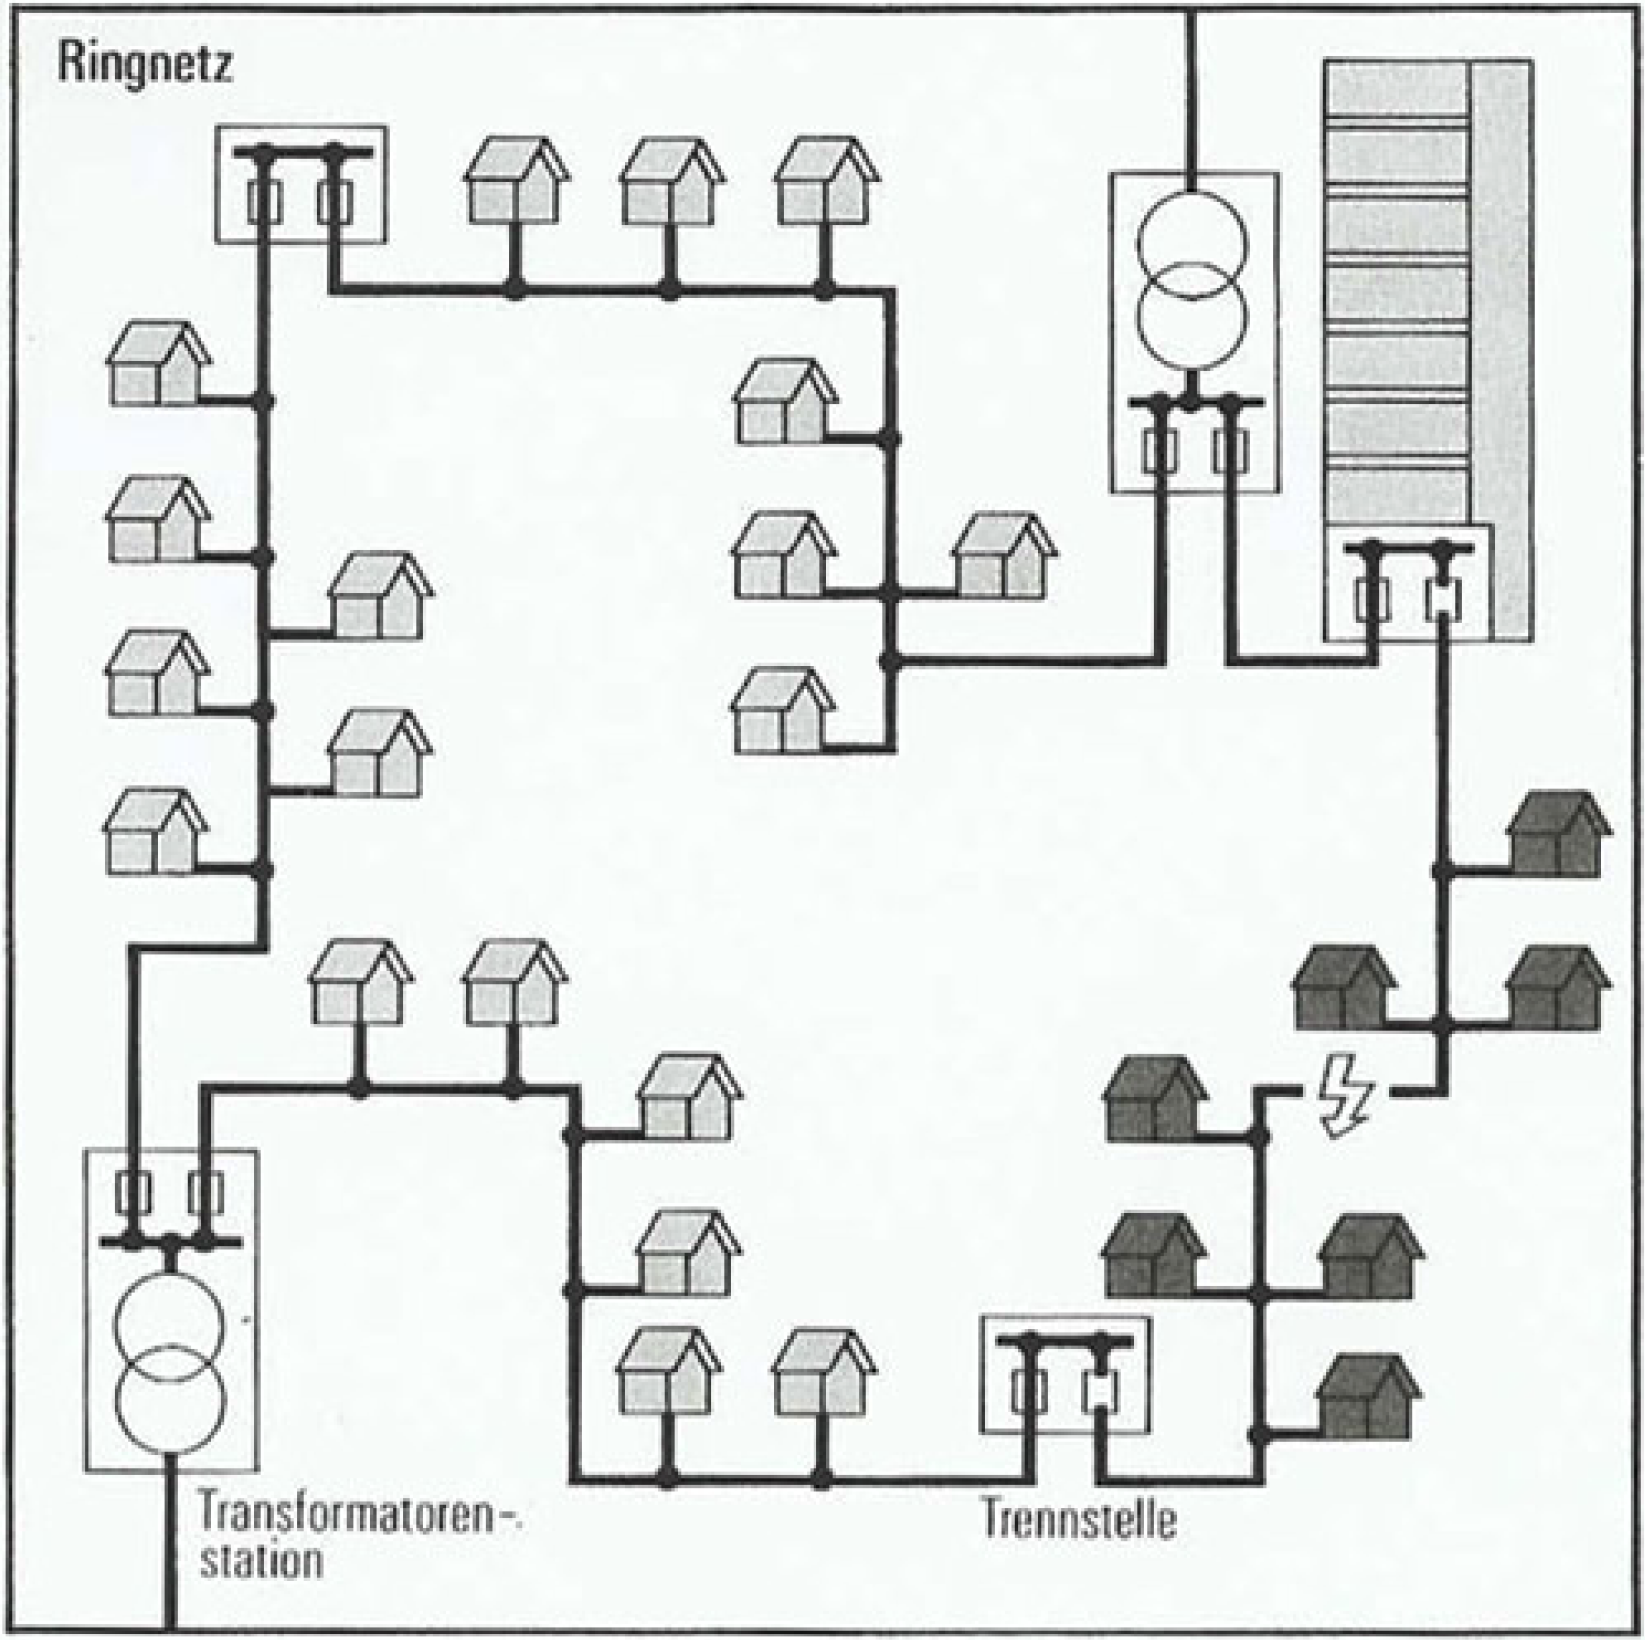
\includegraphics[width=0.55\columnwidth, align=c]{images/Ringnetz.png}

% \textbf{Pro:}
% \begin{itemize}
%     \item höhere Versorgungssicherheit
%     \item geringere Verluste
%     \item verbesserte Spannungshaltung
% \end{itemize}

% \vspace{1em}
% \textbf{Contra:}
% \begin{itemize}
%     \item höhere Anspruch an die Qualifikation des Wartungspersonals
% \end{itemize}

\subsection{Maschennetz}
    \begin{minipage}[t]{0.5\columnwidth}
        \begin{itemize}
            \pro eine optimale Versorgungszuverlässigkeit
            \pro optimale Spannungshaltung
            \pro minimale Leistungsverluste
        \vspace{1em}
            \con hohe Investitionskosten
            \con hohe Projektions- und Wartungsaufwand
            \con höhere Kurzschlussströme
        \end{itemize}
    \end{minipage}%
    \hfill
    \begin{minipage}[t]{0.45\columnwidth}
        \centering \vspace{-0.7\baselineskip}
        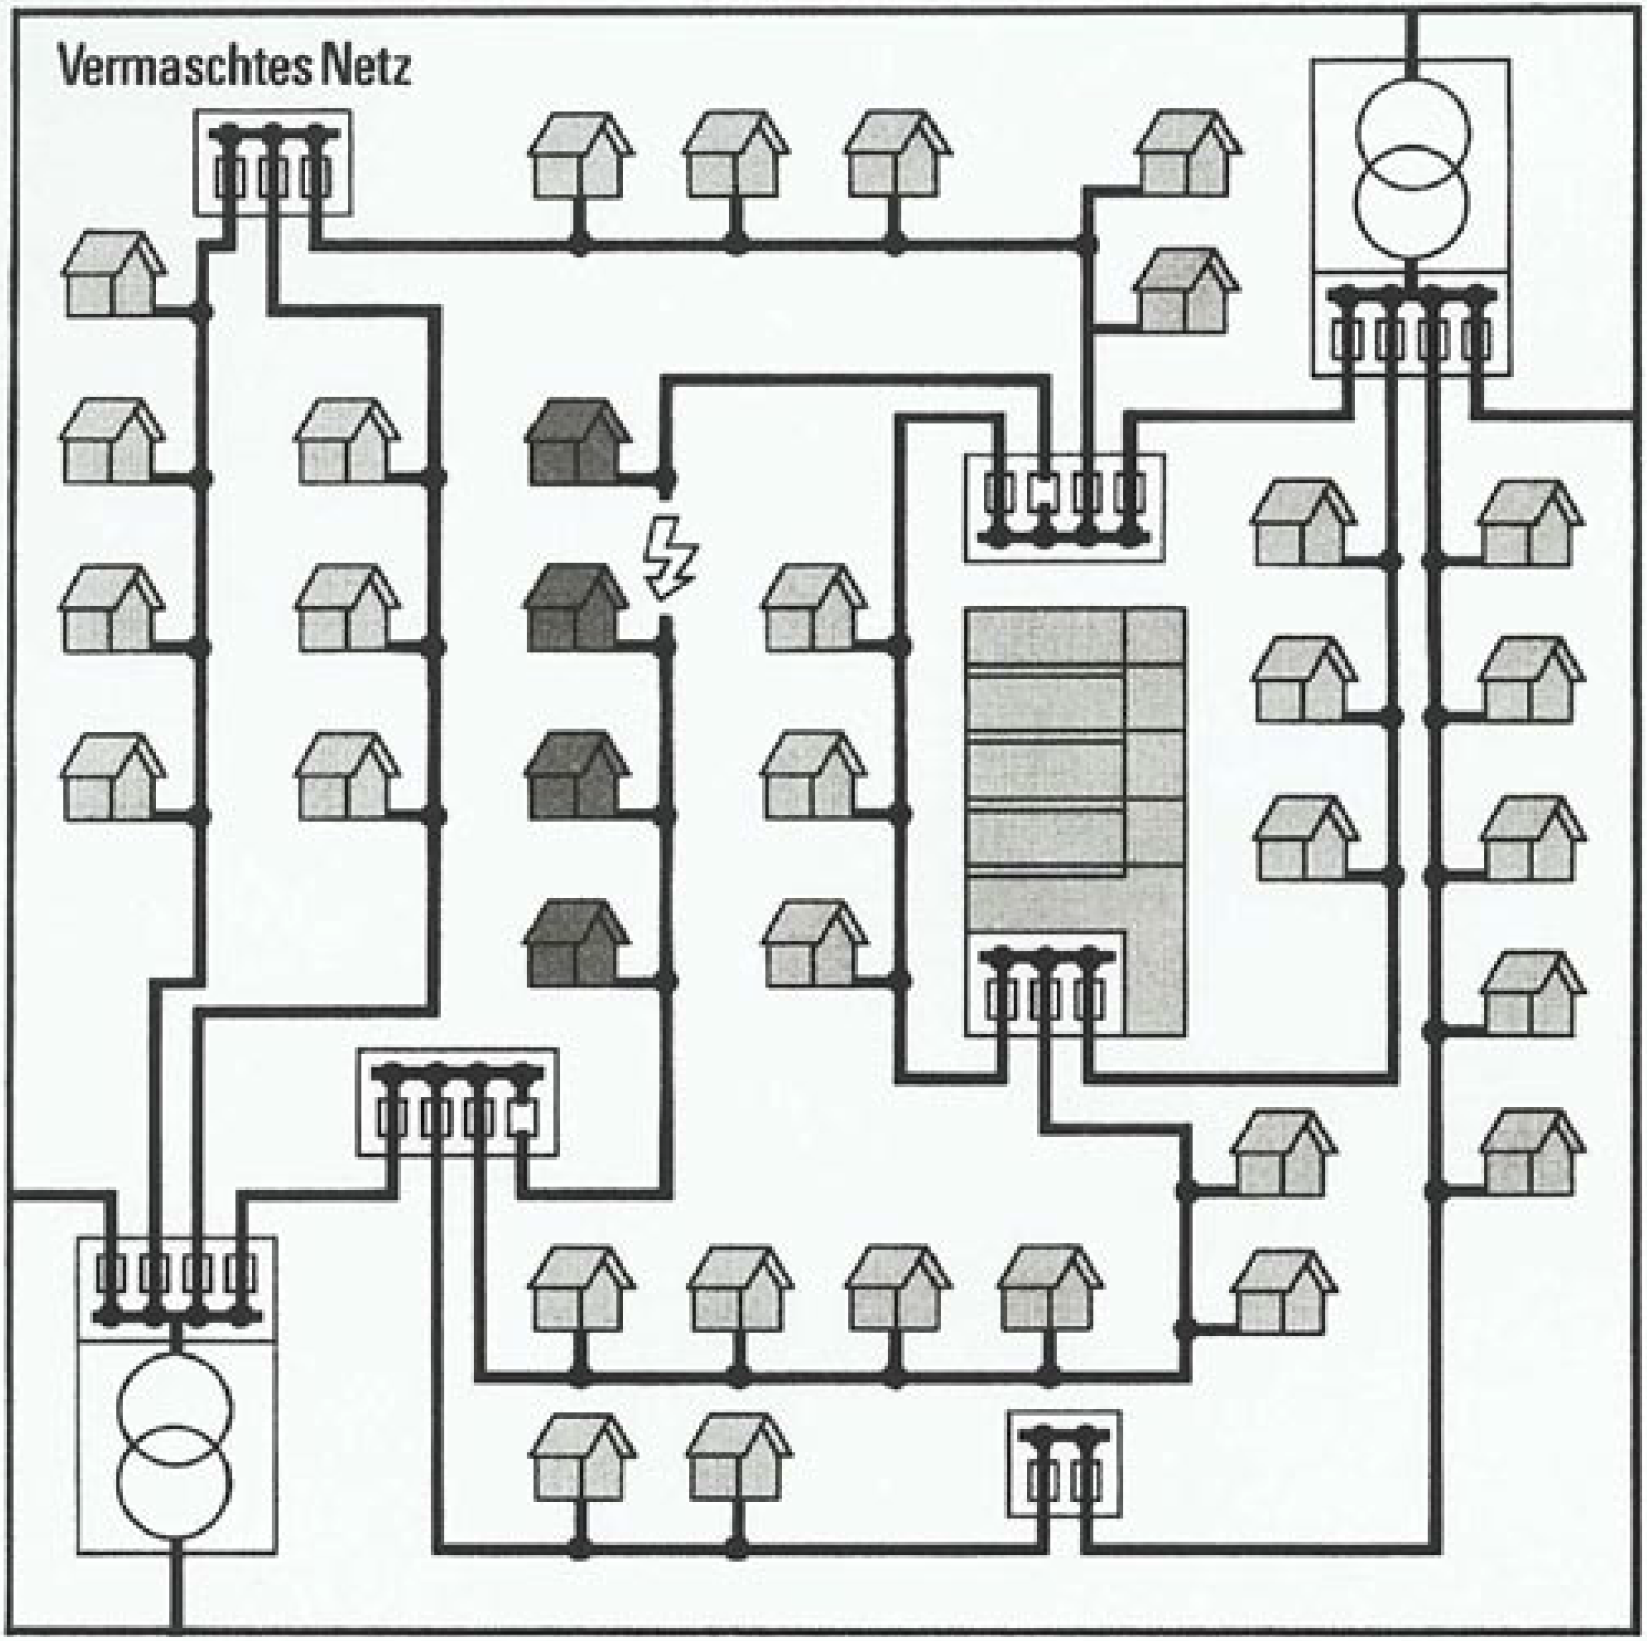
\includegraphics[width=0.9\textwidth]{images/Maschennetz.png}
    \end{minipage}

% 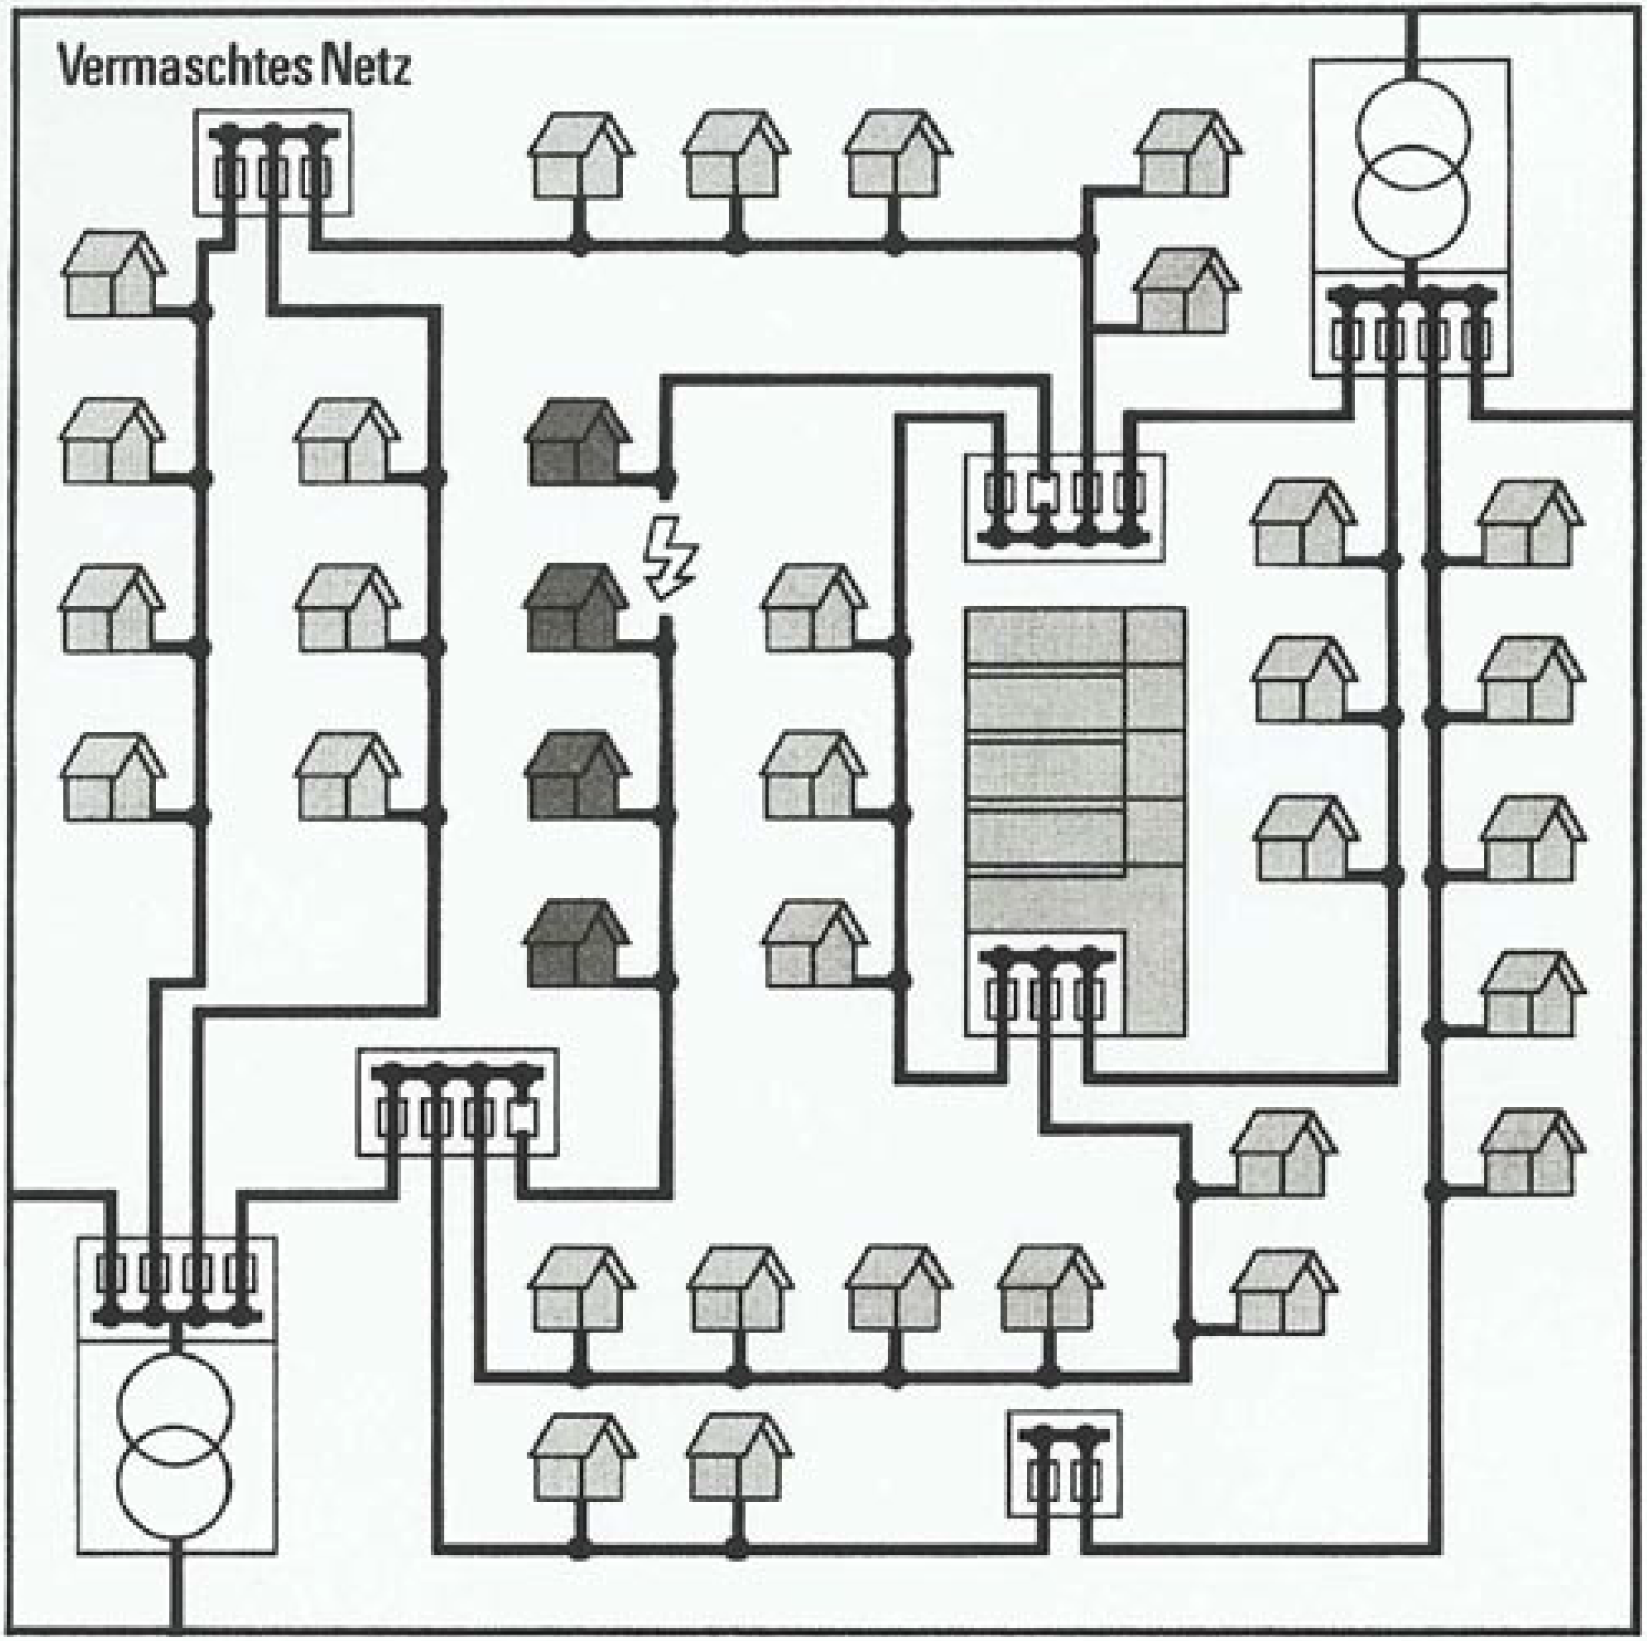
\includegraphics[width=0.55\columnwidth, align=c]{images/Maschennetz.png}

% \textbf{Pro:}
% \begin{itemize}
%     \item eine optimale Versorgungszuverlässigkeit
%     \item optimale Spannungshaltung
%     \item minimale Leistungsverluste
% \end{itemize}

% \vspace{1em}
% \textbf{Contra:}
% \begin{itemize}
%     \item hohe Investitionskosten
%     \item hohe Projektions- und Wartungsaufwand
%     \item höhere Kurzschlussströme
% \end{itemize}